\section{Wandler}

\subsection{Kennlinien\hartl{432}}
\begin{tabular}{|>{\bfseries}p{0.31\textwidth}|c|c|}
	\hline
	& \textbf{ADC} & \textbf{DAC} 
	\\ \hline
	Kennlinien idealer Wandler
	& \parbox[c][6cm]{0.31\textwidth}{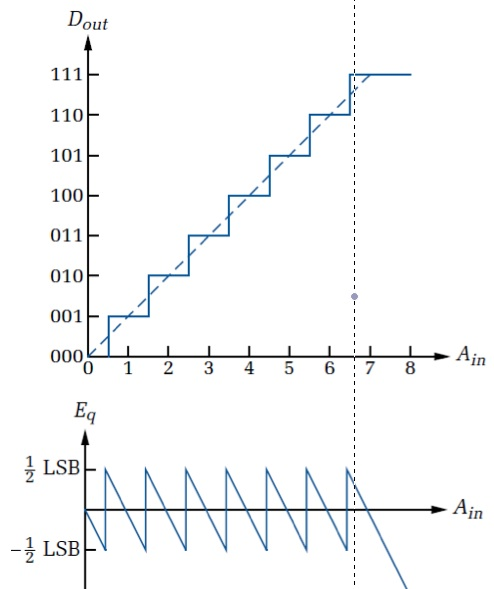
\includegraphics[height=5.9cm]{./pictures/idealerADC.jpg}}
	& \parbox[c]{0.31\textwidth}{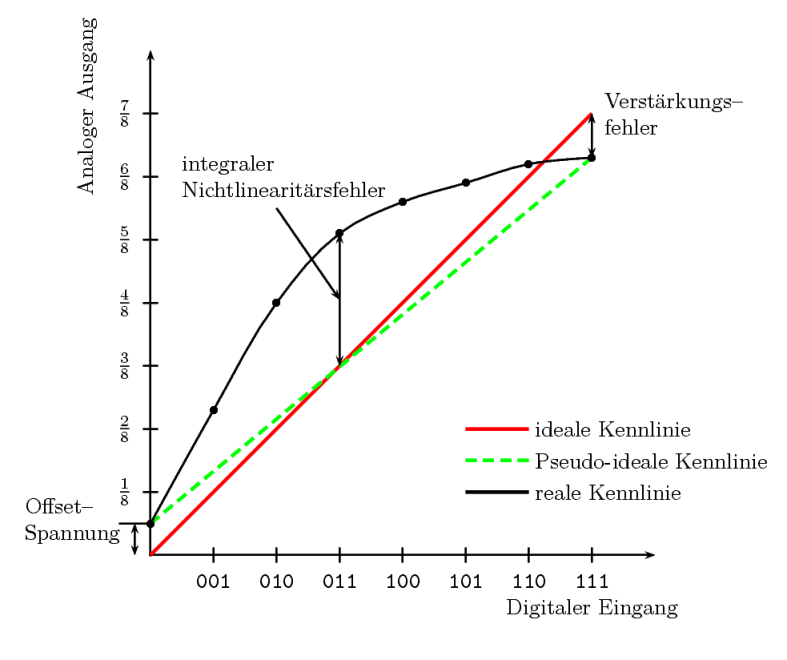
\includegraphics[width=0.31\textwidth]{./pictures/idealerDAC.png}}
	\\ \hline
	Quantisierungsintervall
	& $q = \frac{A_{max}}{2^N} = \frac{V_{refp}-V_{refn}}{2^N}$
	& $q = \frac{A_{Ref}}{2^N} = 1LSB $
	\\ \hline
	Quantisierungsfehler
	& $ -\frac{q}{2}\leq E_{q}<+\frac{q}{2} $
	&
	\\ \hline 
	Ausgangsgrösse
	&
	& $A_{out} = D_{in}\cdot q = D_{in}\cdot(\frac{A_{Ref}}{2^N})$
	\\ \hline
	Offset-Fehler \hartl{434}
	& 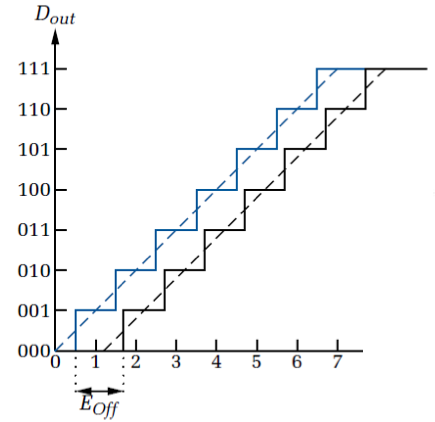
\includegraphics[height=3cm, trim=0cm 0cm 6.2cm 6.5cm, clip=true, valign=t]{./pictures/EoffADC.png}
	& 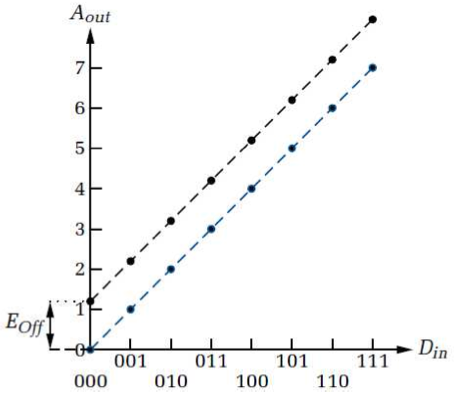
\includegraphics[height=3cm, trim=0cm 0cm 6cm 6.5cm, clip=true, valign=t]{./pictures/EoffDAC.png}
	\\ \hline
	Verstärkungsfehler\hartl{436}
	& 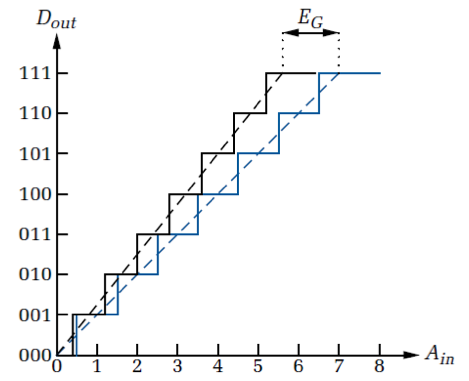
\includegraphics[height=3.8cm, valign=t]{./pictures/verstaerkungsfehlerADC.png} 
    & 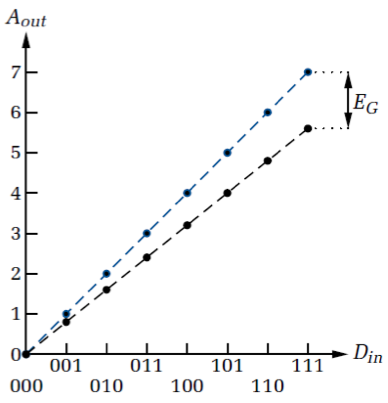
\includegraphics[height=3.8cm, valign=t]{./pictures/verstaerkungsfehlerDAC.png}
	\\ \hline
	Differentielle Nichtlinearität DNL \hartl{437}
	& 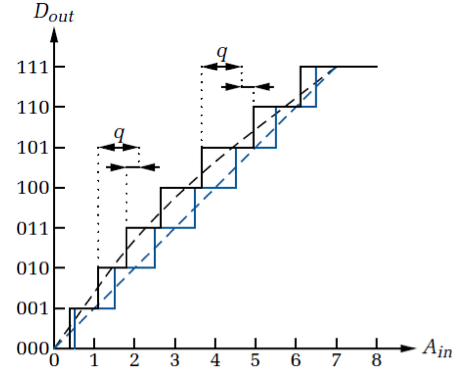
\includegraphics[height=3.8cm, valign=t]{./pictures/DNL_ADC.png}
	& 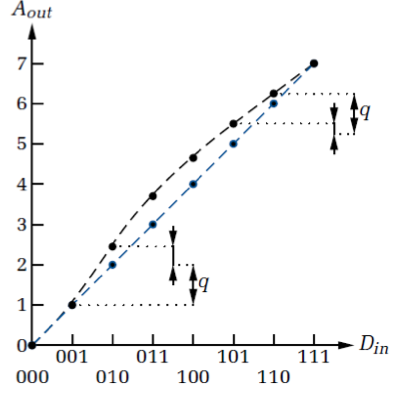
\includegraphics[height=3.8cm, valign=t]{./pictures/DNL_DAC.png}
	\\ \hline
	Integrale Nichtlinearität INL \hartl{439}
	& 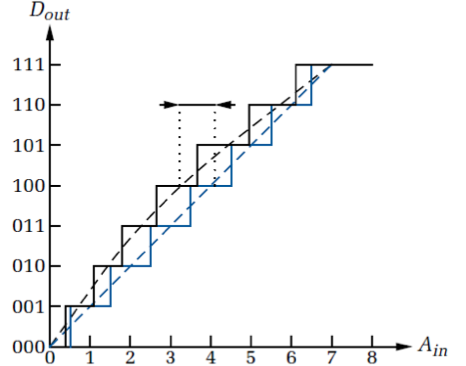
\includegraphics[height=4cm, valign=t]{./pictures/INL_ADC.png}
	& 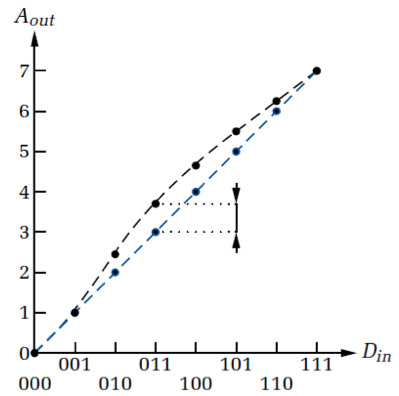
\includegraphics[height=4cm, valign=t]{./pictures/INL_DAC.png}
	\\ \hline
\end{tabular}

\subsection{Eigenschaften und Fehler bei dynamischen Signalen\hartl{442}}
\subsubsection{Aperturfehler\hartl{442}} 
Bei einer periodischen Abtastung eines Signals ist immer ein gewisse zeitliche
Unsicherheit im Abtastzeitpunkt (Aperturunsicherheit) gegeben. Ist der Aperturfehler grösser als der maximal
auftretende Quantisierungsfehler ($\frac{1}{2}LSB$) so verschlechtert sich die Auflösung des Umsetzers. 


\begin{longtable}[c]{ l  l l l }
\begin{minipage}{4cm}

  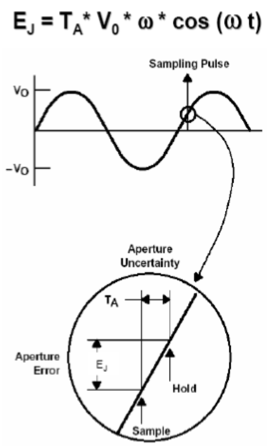
\includegraphics[scale=0.45]{pictures/aperturfehlercos}

\end{minipage}
&
\begin{minipage}{3cm}

  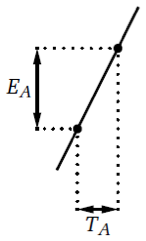
\includegraphics[scale=0.5]{pictures/aperturfehler}
\end{minipage}
&
\begin{minipage}{5cm}
\begin{gather*}
x(t)=S\sin(2\pi ft)\\
\dot{x}(t)=2\pi fS\cos(2\pi t)\\
max\mid\dot{x}(t)\mid= 2\pi fS \\
E_{A}=2\pi fST_{A}\\
2S=A_{Ref}\\
E_{A}<E_{q}\\
E_{q}=\frac{q}{2}=\frac{A_{Ref}}{2\cdot2^N}\\
E_{A}<\frac{A_{Ref}}{2\cdot2^N}\\
2\pi fST_{A} <\frac{2S}{2\cdot2^N}\\
T_{A}\frac{1}{\pi f2^{N+1}}
\end{gather*}
\end{minipage}

&
\begin{minipage}{5cm}
\begin{tabular}{ll}
$E_{A}$: &Aperturfehler\\
$E_{q}$:&Quantisierungsfehler\\
$T_{A}$:&Zeitfehler\\
$A_{Ref}$:&analoge Referenz\\
N:& N bit Auflösung\\
S: &Amplitude\\
f: &Frequenz\\
t: &Zeit\\
x(t):&Signal
\end{tabular}


\end{minipage}
\\
\end{longtable}


\subsubsection{Aliasing\hartl{444}}
Aliasing entsteht bei Unterabtastung, d.h wenn das Abtasttheorem verletzt wird.
Es entstehen falsche, nur scheinbar vorhandene Komponenten im zeitdiskreten
Signal.

\begin{tabular}{llll}
	\textbf{Abtasttheorem}
	& $f_{S}>2f_{max}$
	& $f_{s}$: Abtastfrequenz
	&$f_{max}$:max. Frequenz des Signals
\end{tabular}

\subsection{Lineares Modell der Quantisierung\hartl{448}}
\subsubsection{Signal-Rausch-Verhältnis\hartl{450}}
\begin{multicols}{2}
\begin{align*}
P_{Sig} &= S^2_{Eff} = \frac{S^2}{2} = \frac{(\frac{A_{Ref}}{2})^2}{2} = \frac{A^2_{Ref}}{8}\\
P^2_{N} &= \frac{q^2}{12} = \frac{(\frac{A_{Ref}}{2^N})}{12} = \frac{A^2_{Ref}}{12\cdot2^{2N}}\\
SNR		&= \frac{P^2_{S}}{P^2_{N}} = \frac{\frac{A^2_{Ref}}{8}}{\frac{A^2_{Ref}}{12\cdot2^{2N}}} = \frac{12\cdot2^{2N}}{8} = 3\cdot2^{2N-1}\\
SNR_{dB}&= 10\log(3\cdot2^{2N-1}) = 6.02N+1.76dB\\
ENOB	&= \frac{SNR_{dB}-1.76}{6.02}
\end{align*}

\begin{tabular}{ll}
$P_{Sig}$:&Signalleistung\\
SNR:&Signal-Rausch-Verhältnis\\
$SNR_{dB}$:&Signal-Rausch-Verhältnis in dB\\
ENOB:&Effektive Anzahl Bits\\
\end{tabular}
\end{multicols}